\section{Likformig rörelse}
En likformig rörelse är en rörelse som genomförs med konstant hastighet i jämvikt. Den kan egentligen sammanfattas med den så kallade ''SVT-trianglen'':
\begin{figure*}[h]
    \centering
    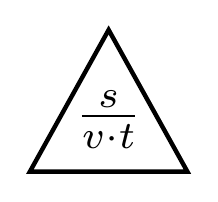
\begin{tikzpicture}[scale=2, every node/.style={scale=2}]
        \draw[ultra thick] (-0.5,-0.5) -- (0,-0.5) node[anchor=south, align=center] {\(\frac{s}{v \cdot t}\)} -- (0.5,-0.5) -- (0,0.4) -- cycle;
    \end{tikzpicture}
\end{figure*}

Denna kan användas genom att täcka för den sökta enheten med ett finger. och sedan kommer formel för den övertäcka enheten bli kvar. Sammanfattat gäller följande formler:
\begin{align*}
    s &= v \cdot t \\
    v &= \frac{s}{t} \\
    t &= \frac{s}{v} \\
\end{align*}

\section{Likformigt accelererande rörelse}
Om hastigheten inte längre är konstant är den enklaste nästa steg att accelerationen $a$ är konstant. då gäller följande formler:
\begin{align*}
    s &= \frac{at^2}{2} + v_0t + s_0 \\
    v &= at + v_0 
\end{align*}

\section{Allmän rörelse}
All rörelse kan beskrivas med hjälp av de ovanstående formlerna men man måste blanda in lite integral- och differentialkalkyl. För att uppnå denna fullständinga definition vill vi först tänka på rörelsens storheter som funktioner av tiden:
\begin{equation*}
    s(t) \text{ för sträcka, } v(t) \text{ för hastighet och } a(t) \text{ för accelration.}
\end{equation*}
Med detta kan vi sedan beräkna deras relation i alla möjliga fall. Här antar jag att du är bekant med tanken bakom integraler och derivator så här är snabbversionen av alla generella formler givet att $a(t)$ är linjärt:
\begin{align*}
    s(t) &= \frac{kt^3}{6} + \frac{a_0t^2}{2} + v_0t + s_0 \\
    v(t) &= \frac{kt^2}{2} + a_0t + v_0 \\
    a(t) &= kt + a_0
\end{align*}
eftersom
\begin{align*}
    v(t) &= s'(t) \\
    a(t) &= v'(t) = s''(t) \\
    s(t) &= \int{v(t)}\, dt = \iint{a(t)}\, dt\, dt
\end{align*}
(Om du inte tycker detta räcker finns en fullständig härledning i bilaga \ref{derive:allmänrörelse}) Utifrån detta kan vi nu beräkna all rörelse bara vi vet formeln för en av storheterna. Om det inte finns en formel ska den hittas experimentellt eller så går det inte. Man kan sätta in valfri funktion för $a(t)$ och om man integrerar korrekt får man ändå rätt svar så detta är verkligen en allmän metod.